\chapter{Agent Negotiation}
\minitoc

\newpage
\begin{itemize}
\item Davis and Smith\\
\say{Negotiation is a process of improving agreement (reducing inconsistency and uncertainty) on common viewpoints or plans through the exchange of relevant information}.\\

Negotiation is a two way exchange of information (more than one agent must be involved for negotiation to happen).\\
Each party evaluates the information from its own perspective.\\
final agreement is achieved by \side{mutual selection}.
\item Pruitt\\
\say{Negotiation is a process by which a joint decision is made by two or more parties. The parties first verbalize contradictory demands and then move towards agreement by a process of concession or search for new alternatives}\\

\side{Mutual conflict} is the necessary condition to start negotiation.\\
Negotiation involves three main elements: \side{communication}, \side{decision making} (decision about next concession to make in order to continue negotiation) and a \side{procedural model} (protocol inside which we communicate and make decision).\\
\side{Implicit negotiation} where one or more parties does not know that there is conflict can happen but it will not be treated in the course.
\end{itemize}

From the definitions provided we can conclude that there are three basic negotiation categories:
\begin{itemize}
\item \side{Negotiation language category} (Communication)

We will consider the language category more in depth in chapter \ref{ch:AgentCommunication}: Agent Communication.\\
The language category deals with the concepts of:
\begin{itemize}
\item \side{Language primitives}\\
Low level communications (message sending) and conversational aspects (relative to speech acts and performatives)
\item \side{Object structure}\\
What is the object of negotiation (price, schedule, tasks, ...) and what is the context of the message/information.
\item \side{Internal protocol}\\
Specify the possibilities of initiating a negotiation cycle and responding to a message
\item \side{Semantics}\\
Strictly related to language primitives (pre-conditions, post-conditions, modal logic).
\end{itemize}

\item \side{Negotiation decision category} (Decision making)

The decision category deals with which strategy and consequently which language primitive to choose inside of a protocol.\\
It deals with the concepts of:
\begin{itemize}
\item preferences\\ 
what are preferrable outcomes
\item utility functions\\
 numerical/functional representation of preferences
\item comparing and matching functions
\item negotiation strategies
\end{itemize}

\item \side{Negotiation process category} (Protocols/procedural model)

It deals with the concepts of:
\begin{itemize}
\item \side{Procedural negotiation model}\\
what is the protocol of negotiation and their properties
\item \side{System behaviour and analysis}\\
analysis of the interaction between different parts of the system in order to recognize what are protocols and preferences (it will not be considered in the course)
\end{itemize}
\end{itemize}
\begin{figure}[!h]
\centering
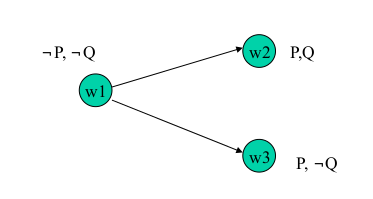
\includegraphics[width=.5\textwidth]{/01/00}
\caption{trivial form of how the categories are interralated in the negotiation context}
\end{figure}

Furthermore, since negotiation happens when mutual conflict occurs, we can say that negotiation is a \side{conflict resolution} approach/method/area.

In general terms, negotiation usually proceeds in \side{series of rounds}  with every agent making a proposal at every round.
For this reason, the negotiation process can be seen as a mutual exchange of information.

\begin{figure}[!h]
\centering
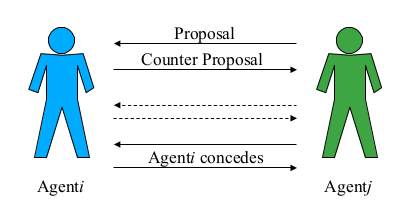
\includegraphics[width=.5\textwidth]{01/01}
\end{figure}

Another way of looking at the negotiation process is as an iterative concession process: each agent starts at its most preferred outcome and makes a proposal, it will then proceed to conceed to a less preferred outcome until a \side{Point of acceptance or agreement} is reached. (Be aware of the fact that not all negotiation end with agreement).

\begin{figure}[!h]
\centering
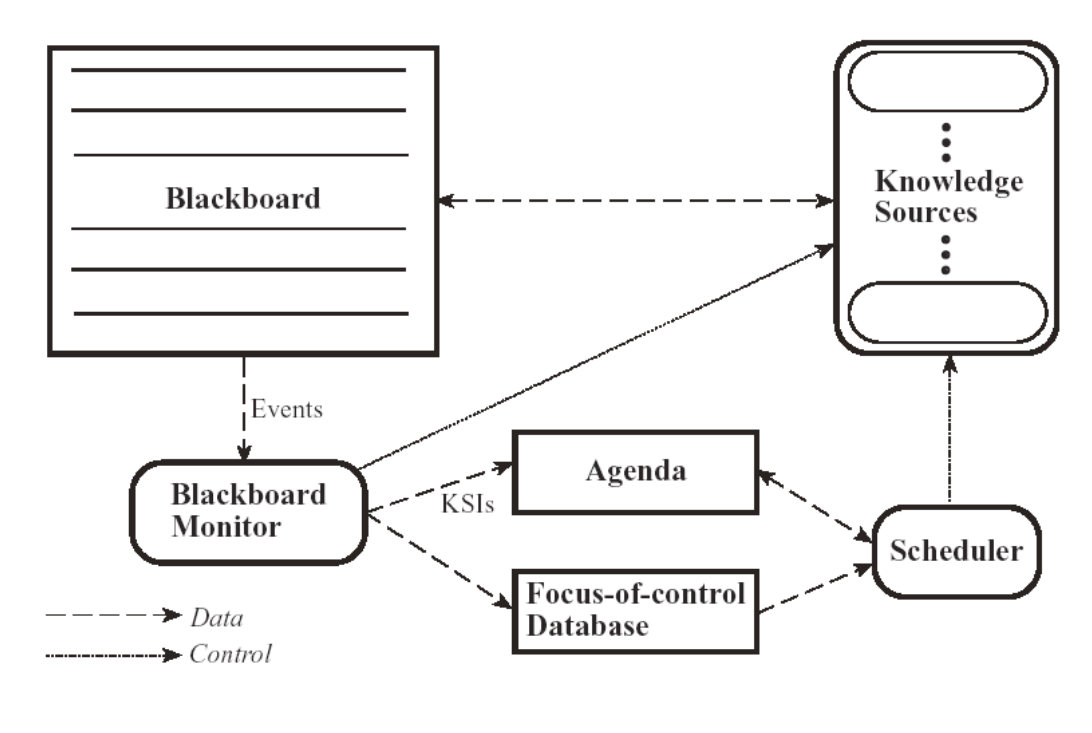
\includegraphics[width=.5\textwidth]{01/02}
\end{figure}

Hence the Negotiation process can be seen as moving towards a point of agreement.

\section{Multiagent Interactions}
	In the typical structure of a multiagent systems, one can notice the presence of some common elements:
	\begin{itemize}
	\item the system contains a number of agents
	\item each agent has the ability to communicate with another agent
	\item each agent has the ability to act in an environment
	\item different agents have different \side{spheres of influence}, i.e. they are able to influence or have control over the environment, or a part of it.
	\item these spheres of interest may coincide or overlap giving rise to dependencies between agents.
	\end{itemize}	
	
	Thus:\\
	\say{When faced with what appears to be a multiagent domain, it is critically important to understand the type of interaction that takes place between agents in order to be able to make the best decision possible about what action to perform.}

\subsection{Utilities and Preferences}
In order to simplify the analysis of multiagent interactions, throughout this chapter we will consider the following assumption, unless stated differently:
	\begin{itemize}
	\item Two agents act and interact in an environment. We will refer to these two agents as agent $i$ and agent $j$
	\item The two agents are \side{self-interest}, i.e. each agent has its own preferences and desires about how the world should be
	\item There exists a \side{set of outcomes} that the two agents have preferences over. We will refer to this set with the notation:
	\[\Omega = \{\omega_1, \omega_2,...\}\]
	\end{itemize}
	
	The preferences of the two agents are formally captured by means of \side{utility functions}, which maps each outcome in the set $\Omega$ to a real number describing how “good” an outcome is.\\
	Since the agents are self-interest each agent will have its own utility function, hence:
	\[u_i\,:\,\Omega\rightarrow\mathbb{R}\qquad;\qquad u_j\,:\,\Omega\rightarrow\mathbb{R}\]
	The introduction of an utility function eventually leads to a \side{preference ordering} over the outcomes of the set for each agent.
	This means that, if $\omega$ and $\omega’$ are both possible outcomes contained in $\Omega$ and $u_i(\omega)\ge u_i(\omega’)$, then agent $i$ preferes outcome $\omega$ at least as much as outcome $\omega’$.
	
	Since we will make extensive use of the concept of preference ordering throughout the next sections, it is worth introduce a much more compact notation. We will write:
	\begin{align*}
	\omega \cge_i \omega’ &&\text{ as an abbreviation for } && u_i(\omega) \ge u_i(\omega’)\\
	\omega \cmore_i \omega’ &&\text{ as an abbreviation for } && u_i(\omega) > u_i(\omega’)
	\end{align*}
	where the second expression represents the case in which outcome $\omega$ is \side{stricly preferred} by agent $i$ over $\omega’$.
	
	In other words, the notation can be summarized as follows:
	\begin{empheq}[box=%
	\fbox]{gather*}
		\omega \cmore_i \omega’ \,\iff\,u_i(\omega)\ge u_i(\omega’)\text{ and not } u_i(\omega)=u_i(\omega’)
	\end{empheq}
	
	Moreover we can notice that the ordering relation expressed by the operator $\cge$, has the following properties:
	\begin{enumerate}
	\item \side{Reflexivity}
	\[\forall \omega \in \Omega\rightarrow \omega\cge_i\omega\]
	\item \side{Transitivity}
	\[\text{If } \omega \cge_i\omega’ \text{ \&\& } \omega’\cge_i\omega`` \rightarrow \omega \cge_i\omega``\]
	\item \side{Comparability}
	\[\forall \omega\in \Omega, \forall \omega’\in\Omega\rightarrow \omega\cge_i\omega’\text{ || } \omega’\cge_i\omega\]
	\end{enumerate}
	The strict preference relationship still has the second and third property, however it is not reflexive
	
\subsection{Setting the scene}
So far, we have talked introduced a model to represent the agents preferences, but we still need to formalize a model of the environment in which agents act and interact. In particular, we will assume that:
	\begin{itemize}
	\item Two agents will simultaneously choose an action to perform in the environment
	\item as a result of the actions they select, an outcome in $\Omega$ will result
	\item the \side{actual outcome} that will result will depend on the particular \side{combination of actions} performed.
	
	In other terms: both agents can influence the actual outcome 
	\item The two agents must perform an action
	\item The two agents cannot see the action performed by the other agent
	\end{itemize}
	
	We will restrict our analysis to two possible actions that the agent can choose from: cooperate $C$ and defect $D$. Hence, we will refer to the \side{set of actions} with the notation
	\[Ac = \{C,D\}\]
	Given all the above, the environment formally described by a \side{state transformer function}:
	\[\tau: \underbrace{Ac}{\text{agent $i$’s action}}\times\underbrace{Ac}{\text{agent $j$’s action}}\rightarrow \Omega\]
	Hence, several scenarios can happen:
	\begin{enumerate}
	\item The environment maps each combination of actions to a different outcome, and thus is sensitive to the actions of both agents
	\[\tau(D,D)=\omega_1\qquad\tau(D,C)=\omega_2\qquad\tau(C,D)=\omega_3\qquad\tau(C,C)=\omega_4\]
	\item The environment maps each combination of actions to the same outcome and thus neither of the agents have influence in the environment
	\[\tau(D,D)=\omega_1\qquad\tau(D,C)=\omega_1\qquad\tau(C,D)=\omega_1\qquad\tau(C,C)=\omega_1\]
	\item The environment maps each combination of actions to an outcome that is correlated to the choice of only one agent and thus the outcome depends solely on the action performed by one agent
	\[\tau(D,D)=\omega_1\qquad\tau(D,C)=\omega_2\qquad\tau(C,D)=\omega_1\qquad\tau(C,C)=\omega_2\]	
	\end{enumerate}
	Since the latter two cases are of no interest for our analysis we will focus on the scenario in which both agents exert some kind of influence on the actual outcome. We, therefore, will consider the agent preferences (in the form of utility function) as follows
	\[
	\left.
	\begin{aligned}
	u_i(\omega_1) = 1&\quad u_i(\omega_2) = 1&\quad u_i(\omega_3) = 4&\quad u_i(\omega_4) = 4\\
	u_j(\omega_1) = 1&\quad u_j(\omega_2) = 4&\quad u_j(\omega_3) = 1&\quad u_j(\omega_4) = 4
	\end{aligned}
	\right\}
	\]
	Given the state transformer function, we can abuse notation and write
	\[
	\left.
	\begin{aligned}
	u_i(D,D) = 1&\quad u_i(D,C) = 1&\quad u_i(C,D) = 4&\quad u_i(C,C) = 4\\
	u_j(D,D) = 1&\quad u_j(D,C) = 4&\quad u_j(C,D) = 1&\quad u_j(C,C) = 4
	\end{aligned}
	\right\}
	\]
	Hence, with respect to agent $i$’s preferences (first row) over the possible outcomes, we can characterize the preference ordering as follows:
	\[(C,C) \cge_i(C,D) \cge_i(D,C) \cge_i(D,D) \]
	Similarly for agent $j$, the resulting preference ordering can be characterize as follows:
	\[(C,C) \cge_i(D,C) \cge_i(C,D) \cge_i(D,D) \]
	It is straightforward to see that if both agents \side{act rationally}, i.e. \say{they both choose to perform the action that will lead to their preferred outcomes}\cite{mastxt}, they will both choose to cooperate.
	This is because, both agents prefer all the outcomes in which they cooperate, regardless of what the other agent action is.
	
	A common way to represent the previously described interaction scenario is via \side{pay-off matrix} (standard game-theoretic notation):
	\begin{table}[!h]
	\centering
	\begin{NiceTabular}{c|w{c}{0.75cm}w{c}{0.75cm}|w{c}{0.75cm}w{c}{0.75cm}}
	&\Block{1-2}{i defects}&&\Block{1-2}{i cooperates}&\\
	\hline
	\Block{2-1}{j defects}&&1&&4\\
	&1&&1&\\
	\hline
	\Block{2-1}{j cooperates}&&1&&4\\
	&4&&4&
	\end{NiceTabular}
	\end{table}
	The pay-off matrix uniquely defines a \side{game in strategic form}. The way to interpret it is as follows:
	\begin{itemize}
	\item each cell in the matrix correspond to one of the possible outcomes
	\item The top-right value in each cell corresponds to the payoff received by the column player
	\item The bottom-left value in each cell corresponds to the payoff received by the row player
	\end{itemize}
	
\subsection{Solution Concepts and Solution Properties}
A question still remains unanswered: What should an agent do? What action should he chooses? 
		
		We briefly touched on the topic on the previous section, but we have provided neither the concepts that make up the solution nor the desirable properties that a solution should have.
		
		In this section, we will tackle the problem to its core.
		
\subsubsection{Dominant strategies - Dominance}
One of the main concept that we will introduce is that of \side{dominance}.
		
		\say{A strategy $s_i$ is [said to be] \textbf{dominant} for player $i$ if, no matter what strategy $s_j$ agent $j$ chooses, $i$ will do at least as well playing $s_i$ as it would doing anything else}\cite{mastxt}.
		The notion of \side{dominant strategy} is strictly related to the concept of \side{best response}, in the sense that \say{a strategy $s_i$ for agent $i$ is dominant if it is the best response to \textbf{all} of agent strategies}\cite{mastxt}.
		
		Thus, a dominant strategy, if it exists, simplify the decision about what action to perform: \say{the agent guarantees its best outcome 
by performing the dominant strategy}\cite{mastxt}.

\subsubsection{Nash Equilibria}
The notion of \side{equilibrium}, or more precisely \side{Nash equilibrium}, is hard to formalize in the context of strategic decision making.
		
		We can, however, provide a basic definition by saying that two strategies $s_1$ and $s_2$ are in Nash equilibrium if:
		\begin{enumerate}
		\item under the assumption that agent $i$ plays $s_1$, agent $j$ can do no better than play $s_2$, and
		\item under the assumption that agent $j$ plays $s_2$, agent $i$ can do no better than play $s_1$
		\end{enumerate}
		From this conditions, one can clearly notice that \textbf{two strategies are in Nash equilibrium if they are the best response to each other}.
		
		The mutual nature of the concept makes it so that \emph{neither agent has any incentive to deviate from a Nash equilibrium}: even if an agent chooses a different strategy, the other agent can do no better than to choose the strategy in Nash equilibrium.
		
		Technically, this type of Nash equilibrium is known as \side{pure strategy Nash equilibrium}, and as much as it is appealing from its theoretical stand point, it is extremely expensive from a computational stand point.\\
		In fact, finding one or more Nash equilibria requires to consider each combination of strategy and check if they are in Nash equilibrium.\\
		Thus, if there are $n$ agents, each with $m$ possible strategies to choose from, the number of possible combinations of actions (and hence possible outcomes) will be $m^n$.
		
		Nonetheless, the presence of Nash equilibrium provides a definite answer to what action an agent should choose. However, two common issues might emerge:
		\begin{enumerate}
		\item Not every interaction scenario has a pure strategy Nash equilibrium
		\item Some interaction scenarios have more than one pure strategy Nash equilibrium
		\end{enumerate}
		
		With regard to the first issue, we need to modify our notion of what a strategy is. So far, we have implicitly considered a strategy as a deterministic choice of an action. This is inline with the fact that the subroutines that an agent can execute should not be subject to uncertainties or randomness (in general, we would like a subroutine to yield the same correct result on different execution).
		
		However, \say{it can be useful to introduce randomness or uncertainty into our actions}\cite{mastxt}.
		The reason why that is can be best explained considering the game or rock-paper-scissors, of which the pay-off matrix is provided below:
		\begin{table}[!h]
		\centering
		\begin{NiceTabular}{c|w{c}{0.75cm}w{c}{0.75cm}|w{c}{0.75cm}w{c}{0.75cm}|w{c}{0.75cm}w{c}{0.75cm}}
		&\Block{1-2}{i plays rock}&&\Block{1-2}{i plays paper}&&\Block{1-2}{i plays scissors}&\\
		\hline
		\Block{2-1}{j plays rock}&&0&&1&&-1\\
		&0&&-1&&1&\\
		\hline
		\Block{2-1}{j plays paper}&&-1&&0&&1\\
		&1&&0&&-1&\\
		\hline
		\Block{2-1}{j plays scissors}&&1&&-1&&0\\
		&-1&&1&&0&
		\end{NiceTabular}
		\end{table}
		From the provided payoff matrix, one can clearly notice that the game has no pure strategy Nash equilibrium as well as no dominant strategy.
		Yet, this is not completely true: a \side{mixed strategy} allows the agent to choose between possible choices by introducing randomness into the selection.\\
		If the agent chooses one of the actions at random, with each choice having equal probability of being selected, the strategy turns out to be in \textbf{Nash equilibrium with itself}. This is because if an agent decides to choose an action at random, the other agent can do no better than adopting the same strategy and vice versa.
		
		In general, if a player has $k$ possible choices, $s_1, s_2, ..., s_k$, then a mixed strategy over these choices takes the form:
		\begin{itemize}
		\item play $s_1$ with probability $p_1$
		\item play $s_2$ with probability $p_2$
		\item ...
		\item play $s_k$ with probability $p_k$
		\end{itemize}
		In other terms, a mixed strategy over $s_1, s_2, ..., s_k$ is a probability distribution over $s_1, s_2, ..., s_k$.
		
		The result formalized by John Forbes Nash, Jr. best summarize the discussion that we have made so far:\\
		\say{Every game in which every player has a finite set of possible strategies has a Nash equilibrium in mixed strategies}
		
\subsubsection{Pareto efficiency}
The notion of \side{Pareto efficiency} or \side{Pareto optimality}, contrary to the notion of Nash equilibrium and dominant strategy, is more of a (desirable) property of solutions rather than a solution concept.
		
		Formally:\\
		\say{an outcome is Pareto efficient if there is no other outcome that improves one player’s utility without making somebody else worse off}.\cite{mastxt}\\
		On the other hand:
		\say{An outcome is said to be Pareto inefficient if there is another outcome that makes at least one player better off without making anybody else worse off}\cite{mastxt}.
		
		To put it in simpler terms we can consider an example: a brother and a sister have to divide a cake. Among the solutions of this problem, those who are Pareto efficient are:
		\begin{itemize}
		\item The brother eats the whole cake
		\item The sister eats the whole cake
		\item Any other distribution of the cake, which leaves no cake left
		\end{itemize}
		Hence, a solution is Pareto efficient if it consumes/uses the total utility.
		
\subsubsection{Maximizing social welfare}
Similarly to Pareto efficiency, \side{social welfare} is an important property of outcomes, but is not generally a way of directly selecting them.
		
		The core principle of \side{Maximizing social welfare} involves the measurement of how much utility is created by an outcome in total.\\
		Formally, let $sw(\omega)$ denote the sum of utilities of each agent for outcome $\omega$
		\[sw(\omega) =\sum_{i\in Ag} u_i(\omega)\]
		the outcome that maximized social welfare is the one that maximizes this value.
		
		From an individual agent’s point of view, the problem with maximizing social welfare is that it does not look at the pay-offs of individual agents, only to the total welfare created. (maximizing social welfare does not care about how the utility of an outcome is divided among the players).


\subsubsection{Other minor properties}
\begin{itemize}
\item \side{Convergence/ guaranteed success}\\
If it ensures that eventually agreement is certain to be reached.
\item \side{Computational efficiency}\\
As little computations is needed as possible. Trade off between the cost of the process and the solution quality
\item \side{Distribution}\\
All else being equal, distributed protocols should be preferred to avoid a single point of failure and a performance bottleneck. This may conflict with minimizing the amount of communication that is required.
\item \side{Stability}\\
Among self interested agents, mechanism should be designed to be stable (non-manipulable), it should motivate each agent to behave in the desired manner.
\item \side{Individual rationality}\\
Participation in a negotiation is individually rational to an agent if the agent's payoff in the negotiated solution is no less than payoff that the agent would get by not participating in the negotiation.\\
A mechanism is individually rational if participation is individually rational for all agents.\\
If the negotiated solution is not individually rational for some agent then self-interested agent would not participate in that negotiation.
\end{itemize}
\subsection{Competitive and Zero-Sum Interactions}
A scenario in which an outcome $\omega\in\Omega$ is preferred by agent $i$ over an outcome $\omega’$, if ,and only if, $\omega’$ is preferred over $\omega$ by agent $j$, is said to be \side{strictly competitive}.\\
	Formally, a competitive scenario takes the form:
	\[\omega \cmore_i \omega’\qquad\iff\qquad\omega’\cmore_j \omega\]
	Under this condition, it is straightforward to see that the preferences of the players are \side{diametrically opposed} to one another
	
	\side{Zero-sum encounters}, similarly, are those in which, for any particular outcome, the utilities of the two agents sum to zero. Formally, these scenario is described by the condition:
	\[u_i(\omega) + u_j(omega) = 0\qquad \forall \omega \in \Omega\]
	Once again, any zero-sum scenario is strictly competitive, allowing for no possibility of cooperative behavior: \say{the best outcome for an agent is the worst outcome for its opponent. If an agent allows the opponent to get a positive utility, then it will get negative utility.}\cite{mastxt}\\
	Popular Zero-sum encounters are the games of chess and checkers as well as rock-paper-scissors.
	
	Interesting enough, zero-sum is debatable that zero-sum games actually exists in real-world scenarios (apart from artificially forms of interaction like the games mentioned before). However, it appears that people interacting in many scenarios have a tendency to treat them as if they were zero sum.
	
\subsection{The Prisoner's Dilemma}
The \side{Prisoner’s Dilemma} is as follows:
	\say{Two man are collectively charged with a crime and held in separate cells. They have no way of communicating with each other or making any kind of agreement. The two man are told that:
	\begin{enumerate}
	\item If one of them confesses to the crime and the other does not, the confessor will be freed, and the other will be jailed for three years
	\item If both confess to the crime, then each will be jailed for two years
	\end{enumerate}
	Both prisoners know that if neither confesses, then they will each be jailed for one year.}\cite{mastxt}
	Under this conditions let us associate the act of confessing with defection $D$ and not confessing with coopering $C$.
	
	There exists 4 possible outcomes to the prisoner’s dilemma:
	\begin{table}[!h]
	\centering
	\begin{NiceTabular}{c|w{c}{0.75cm}w{c}{0.75cm}|w{c}{0.75cm}w{c}{0.75cm}}
	&\Block{1-2}{i defects}&&\Block{1-2}{i cooperates}&\\
	\hline
	\Block{2-1}{j defects}&&2&&0\\
	&2&&5&\\
	\hline
	\Block{2-1}{j cooperates}&&5&&3\\
	&0&&3&
	\end{NiceTabular}
	\end{table}
	Where the number displayed are NOT the year spent in prison.
	
	From the provided payoff matrix we can come up with the preference ordering of each agent/prisoner:
	\[
	\begin{dcases}
	(D,C) \cmore_i (C,C) \cmore_i (D,D) \cmore_i (C,D) & \text{for agent }i\\
	(C,D) \cmore_j (C,C) \cmore_j (D,D) \cmore_j (D,C) & \text{for agent }j\\
	\end{dcases}
	\]
	Thus, we can analyze the best response of an agent to the choice of action of the other:
	\begin{itemize}
	\item Assuming the other player cooperates. The best response is to defect
	\item Assuming the other player defect. The best response is to defect
	\end{itemize}
	From this we can conclude that defection for $i$ is the best response to all possible strategies of the player $j$: by definition, defection is thus a dominant strategy for $i$.
	
	Since the same conclusion can be drawn for agent $j$, the scenario under consideration is \side{symmetric}: this will result in both agent choosing to defect.\\
	From an analysis of the problem under the concepts that we have seen previously, we can state that
	\begin{itemize}
	\item the pair $(D,D)$ is the only Nash equilibrium of the scenario, however intuition says that this is not the best the players can do. 		\item the pair of actions $(D,D)$ is also the only one that is not Pareto efficient. 
	\item The outcome that maximizes social welfare is $(C,C)$
	\end{itemize}
	
	\say{The fact that utility seems to be wasted here, and that the agents could both do better by cooperating, even though the rational thing to do is to defect, is why this is referred to as dilemma.} \cite{mastxt}
	
	Moreover, the prisoner’s dilemma also seems to be the game that characterized the \side{tragedy of the commons}: which is concerned with the use of a shared, depletable resource by a society of self-interested individuals (e.g. overfishing in the seas, exploitation of bandwidth capacity on the Internet).
	
	Many people find the conclusion of the analysis deeply upsetting: \say{the result seems to imply that cooperatoin can only arise as a result of irrational behavior, and that cooperative behavior can be exploited by those who behave rationally.}\cite{mastxt}\\
	Binmore argues that the discomfort we have with the analsys of the prisoner’s dilemma is misplaced:\\
	\say{A whole generation of scholars swallowed the line that the prisoner’s dilemma embodies the essence of the problem of human cooperation. They therefore set themselves the hopeless task of giving reasons why [this analysis] is mistaken... Rational players don’t cooperate in the prisoner’s dilemma because the conditions necessary for rational cooperation are absent}.
	
\subsection{Other Symmetric 2$\times$2 Interactions}
The prisoner’s dilemma and its variation are not the only type of multiagent interaction that exists.
	
	In fact, if we restrict our attention to interaction in which there are:
	\begin{itemize}
	\item Two agents
	\item Each agent has two possible actions (C or D)
	\item The scenario is symmetric
	\end{itemize}
	Then $4! = 24$ possible orderings of preferences, and as a consequence, 24 different games, can be constructed.
	
	\begin{table}[!h]
	\centering
	\begin{NiceTabular}{lll}[hvlines]
	\textbf{Scenario}&\textbf{Preferences over outcomes}&\textbf{Comment}\\
	1&$(C,C)\cmore_i(C,D)\cmore_i(D,C)\cmore_i(D,D)$&cooperation dominates\\
	2&$(C,C)\cmore_i(C,D)\cmore_i(D,D)\cmore_i(D,C)$&cooperation dominates\\
	3&$(C,C)\cmore_i(D,C)\cmore_i(C,D)\cmore_i(D,D)$&\\
	4&$(C,C)\cmore_i(D,C)\cmore_i(D,D)\cmore_i(C,D)$&stag hunt\\
	5&$(C,C)\cmore_i(D,D)\cmore_i(C,D)\cmore_i(D,C)$&\\
	6&$(C,C)\cmore_i(D,D)\cmore_i(D,C)\cmore_i(C,D)$&\\
	7&$(C,D)\cmore_i(C,C)\cmore_i(D,C)\cmore_i(D,D)$&\\
	8&$(C,D)\cmore_i(C,C)\cmore_i(D,D)\cmore_i(D,C)$&\\
	9&$(C,D)\cmore_i(D,C)\cmore_i(C,C)\cmore_i(D,D)$&\\
	10&$(C,D)\cmore_i(D,C)\cmore_i(D,D)\cmore_i(C,C)$&\\
	11&$(C,D)\cmore_i(D,D)\cmore_i(C,C)\cmore_i(D,C)$&\\
	12&$(C,D)\cmore_i(D,D)\cmore_i(D,C)\cmore_i(C,C)$&\\
	13&$(D,C)\cmore_i(C,C)\cmore_i(C,D)\cmore_i(D,D)$&game of chicken\\
	14&$(D,C)\cmore_i(C,C)\cmore_i(D,D)\cmore_i(C,D)$&prisoner’s dilemma\\
	15&$(D,C)\cmore_i(C,D)\cmore_i(C,C)\cmore_i(D,D)$&\\
	16&$(D,C)\cmore_i(C,D)\cmore_i(D,D)\cmore_i(C,C)$&\\
	17&$(D,C)\cmore_i(D,D)\cmore_i(C,C)\cmore_i(C,D)$&\\
	18&$(D,C)\cmore_i(D,D)\cmore_i(C,D)\cmore_i(C,C)$&\\
	19&$(D,D)\cmore_i(C,C)\cmore_i(C,D)\cmore_i(D,C)$&\\
	20&$(D,D)\cmore_i(C,C)\cmore_i(D,C)\cmore_i(C,D)$&\\
	21&$(D,D)\cmore_i(C,D)\cmore_i(C,C)\cmore_i(D,C)$&\\
	22&$(D,D)\cmore_i(C,D)\cmore_i(D,C)\cmore_i(C,C)$&\\
	23&$(D,D)\cmore_i(D,C)\cmore_i(C,C)\cmore_i(C,D)$&defection dominates\\
	24&$(D,D)\cmore_i(D,C)\cmore_i(C,D)\cmore_i(C,C)$&defection dominates
	\end{NiceTabular}
	\end{table}

	For the sake of the analysis we will briefly look into two more of these games: stag hunt and the game of chicken.

\begin{itemize}
\item The stag hunt
\begin{table}[!h]
	\centering
	\begin{NiceTabular}{c|w{c}{0.75cm}w{c}{0.75cm}|w{c}{0.75cm}w{c}{0.75cm}}
	&\Block{1-2}{i defects}&&\Block{1-2}{i cooperates}&\\
	\hline
	\Block{2-1}{j defects}&&1&&0\\
	&1&&2&\\
	\hline
	\Block{2-1}{j cooperates}&&2&&3\\
	&0&&3&
	\end{NiceTabular}
	\end{table}
	
\item The Game of chicken
\begin{table}[!h]
	\centering
	\begin{NiceTabular}{c|w{c}{0.75cm}w{c}{0.75cm}|w{c}{0.75cm}w{c}{0.75cm}}
	&\Block{1-2}{i defects}&&\Block{1-2}{i cooperates}&\\
	\hline
	\Block{2-1}{j defects}&&0&&1\\
	&0&&3&\\
	\hline
	\Block{2-1}{j cooperates}&&3&&2\\
	&1&&2&
	\end{NiceTabular}
	\end{table}
\end{itemize}	


\section{Voting}
So far we have lloked at the general setting of a multiagent encounter. In this section we will look at a specific class of protocols intended for making group decisions. This is the domain of social choice theory (aka voting theory).

\subsection{Social Welfare Functions and Social Choice Functions}
The general setting of a voting protocol is as follows:
\begin{itemize}
\item A set of agents or \side{voters}
\[Ag = \{1, ...,n\}\]
Ideally, this should be finite and the cardinality should be an odd number to avoid ties.
\item A set of possible outcomes or \side{candidates}
\[\Omega =\{\omega_q, \omega_w, ...\}\]
over which voters will make group decision. This set is assumed to be finite.

The goal of the agents is to rank or order these candidates or simply to choose one from the set.
\end{itemize}
The problem that social choice theory tries to solve is,\\
 \say{given a collection of preference orders, one for each agent, how do we combine these to derive a group decision?}.
 
 The answert isby using a \side{social welfare function} which maps the voter preferences to a \side{social preference order}\\
 \[f:\quad \Pi(\Omega) \times ...\times\Pi(\Omega) \rightarrow \Pi(\Omega)\]
 The social preference ordering will be denoted with the notation $\cmore^*$.
 
 If the agents are required to choose just one candidate over the set $\Omega$, we will use a \side{social choice function} or \side{voting procedure}:
 \[f:\quad \Pi(\Omega) \times ...\times\Pi(\Omega) \rightarrow \Omega\]

\subsection{Voting Protocols}
\subsubsection{Simple majority voting}
\begin{itemize}
\item Every voter submits their preference order
\item The winner is the outcome that appears first in the preference orders the largest number of times
\item This is generally applied to single choice, but it can be generalized to a social preference ordering.
\end{itemize}
\side{Simple majority voting} works relatively well with only two candidates, since it is straightforward to implement and understand by the voters.

However, when more than 2 voters are involved problems start to arise.

Let us consider that three voters submitted the following preferences:
\begin{align*}
42\%& \omega_L \cmore \omega_D \cmore \omega_C\\
14\%& \omega_D \cmore \omega_L \cmore \omega_C\\
44\%& \omega_C \cmore \omega_D \cmore \omega_L\\
\end{align*}
Then the winner is selected based on the top preferences (i.e. $C$), even though the majority of the voters considered $C$ as the least preferrable outcome.

This means that in principle the majority of the voters will be unhappy with the result of the voting protocol.

Furthermore, this simple majority protocol is sensible to insincere strategical voting (e.g. the 14\% that voted $D$ instead could have voted for $L$ just to make $C$ lose the voting).

Moreover, the simple majority voting is sensible to \side{Condorcet's paradox}:
\begin{equation*}
\omega_1 \cmore_i \omega_2 \cmore_i \omega_3\\
\omega_3 \cmore_j \omega_1 \cmore_j \omega_2\\
\omega_2 \cmore_k \omega_3 \cmore_k \omega_1\\
\end{equation*}
In this case the winner is dependent on the agenda: which order we start to compute the outcome, but nonetheless $\sfrac{2}{3}$ of the voters will prefer another candidate.

\subsubsection{Binary protocol}
Among the alternative to simple majority voting there is the \side{Binary protocol} (aka sequential majority elections).

\begin{itemize}
\item Voters submit their preference ordering
\item The element of the set of outcomes are compare pairwise
\item the winner of the pairwise ``election'' is allowed to continue to the next pairwise election
\item The order of pairwise elections (i.e. which candidates to compare first), is called \side{agenda}
\end{itemize}

\begin{figure}[!h]
\centering
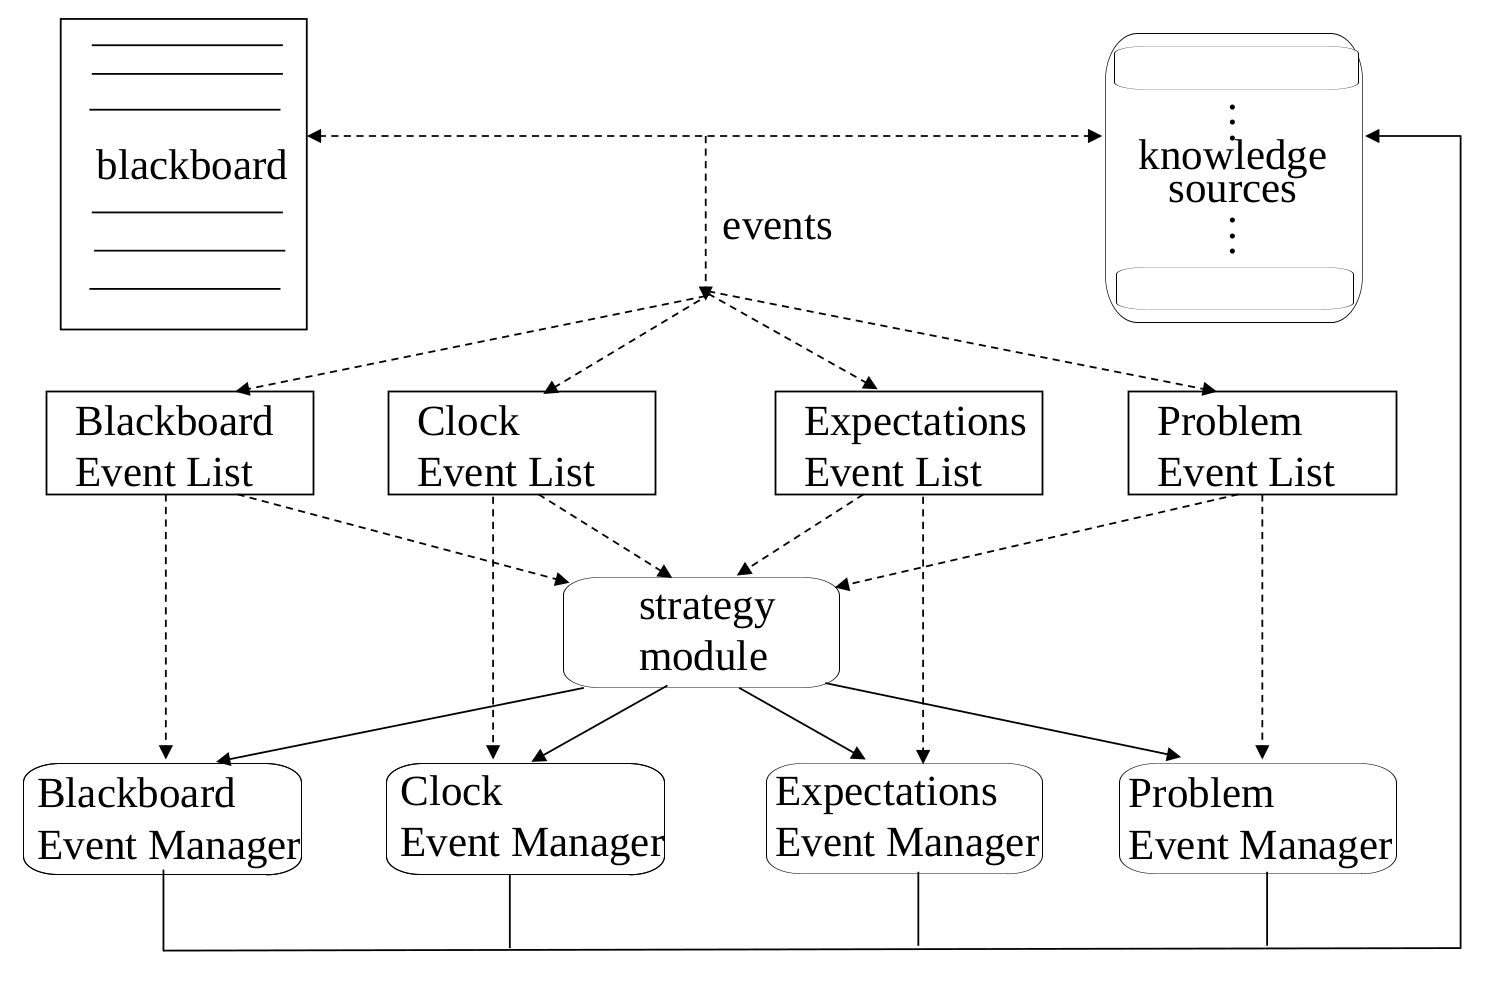
\includegraphics[width= .5\textwidth]{01/03}
\end{figure}


From the picture provided we can clearly notice that the winner of the overall election depends on the agenda, which imply that the protocol can be manipulated if the preference orderings in known a priori.

\subsubsection{Borda protocol}
One issue with simple majority voting and the binary protocol is that they completely ignore the information that is enconded in each submitted preference ordering (they only loop at the top voted candidates).\\
The \side{Borda protocol} addresses such issue:
\begin{itemize}
\item Each voter submit its preference ordering over the candidates
\item a number equal to the cardinality of the set of candidates (i.e. $\abs{\Omega}$) is assigned to the highest candidate in some agent's preference list
\item a value of $\abs{\Omega}-1$ is assigned to the second and so on
\item a the end we sum up the numeric value associated to each preference orderic and obtain the social choice result
\end{itemize}

This protocol is fast when compared to the binary protocol in the case of a large amount of candidates.

However it is not  \side{indipendent of irrelevant alternatives}, i.e. removing one candidate will change the end result.


\subsubsection{Majority Graph: Condorcet's Winner and Slater ranking}
An useful tool to analyse voting procedures or protocols is the \side{Majority Graph}. It can be considered as a succint representation of the voter preferences:
\begin{itemize}
\item each node in the majority graph is a candidate
\item each edge in the majority graph represents a preference (the edge will start from the node most preferred and will terminate in the node less preferred)
\item a \side{possible winner} is a candidate that is the overall winner for at least one agenda. (occurs when there are loops in the majority graph)
\item a \side{Condorcet's winner} is a candidate that is the overall winner for all possible agenda (occurs when there are no loops in the majority graph). In simple terms, is that candidate that will beat all others in a pairwise election.
\end{itemize}

While the overall winner determination is straightforward in the case of a majority graph with no loops (cfr. Condorcet's Winner), it is otherwise in the case of a majority graph with loops.

In that specific scenario, the \side{slater rule} or \side{slater ranking} is considered: it, in fact, tries to find a consistent ranking that does not contain any cycle that is as close a possible to the majority graph.

In other terms, it tries to \say{minimize the number of disagreements between the majority graph and the social choice}.

In practice, the Slater ranking considers the Condorcet's winners obtained by inverting the least amount of edges in the majority graph.
\subsection{Desirable Properties for Voting Procedures}
\begin{enumerate}
\item \side{Pareto condition}\\
There is no other outcome that makes one agent better off without making another agent worse off.

Borda and simple majority voting satisfy this condition.\\
Binary protocol does not (the result depends on the agenda).
\item \side{Condorcet winner condition}\\
The Condorcet winner should be selected by the social choice function.

Only Binary protol satisfies this condition.
\item \side{Indipendence of irrelevant alternatives}\\
Given a set of candidates of which $\omega_i$ and $\omega_j$ are part of. \\
Let us assume that $\omega_i \cmore^* \omega_j$.\\
A change in preferences in any other candidate should not change the relative ranking of $\omega_i$ and $\omega_j$.

None of the protocol we have seen satisfies this property.
\item \side{Dictatorship}\\
A social welfare function is said to be a dictatorship if for some voter $i$ we have
\[f(\bar{\omega_1}, \bar{\omega_2}, ...) = \bar{\omega_i}\]

All protocols we have seen so far are non-dictatorship.
\end{enumerate}

\begin{theorem}[Arrow's theorem]\pside{Arrow's theorem}\\
If $\abs{\Omega}>2$ then the only voting procedure that satisfies Pareto condition, Condercet Winner condition and IIA is dictatorship.
\end{theorem}
\subsection{Insincere Voters}
\begin{itemize}
\item In reality it is seldom that all agent's preferences are known: usually agents have to reveal their preferences.
\item Assuming knowledege of the preferences is equivalent to assuming that the agents reveal their preferences truthfully
\item If an agent can benefit from insincerely declaring his preferences, it will do so.
\item The goal is to generate protocols such that when agents use them according to some stability solution concept (dominant strategy equilibrium) the desirable social outcomes follow
\item The strategies are not externally imposed on the agents, but instead each agent uses the strategy that is best for itself
\end{itemize}
However:\\

Let each agent $i$ from $A$ have some ordering $\theta_i$ from $\Theta$ which totally characterized his preferences. A social choice function $f:\quad \Theta \rightarrow \Omega$ chooses a social outcome given the agent's orderings.

\begin{theorem}[Gibbard-Satterthwaite impossibility theorem]\pside{Gibbard- Satterthwaite impossibility theorem}\\
Let each agent's ordering $\theta_i$ consists of a preference order $\cmore_i$ on $\Omega$.\\
Let there be no restictions on $\cmore_i$ (i.e. each agent may rank the outcomes $\Omega$ in any order).\\
Let $\abs{\Omega} > 2$.\\
Now, if the social function $f(\cdot)$ is truthfully implementable in a dominant strategy equilibrium (or is not manipulable), then $f(\cdot)$ is dictatorial, i.e. there is some agent who gets one of its most preferred outcome chosen no matter what types the other reveal.
\end{theorem}

Broadly speaking, the only procedure or mechanism that is immune to strategic manipulation (in the sense of untruthful report of an agent preference) is dictatorship in the case of more than 2 candidates.

There are ways to circumvent the impossibility theorem, by relaxing the assumptions made by the theorem itself.\\
The individual preferences, in fact, may happen to belong to some restrincted domain, thus invalidating the conditions of the impossibility theorem, and it is known that there are island in the space of agent's preferences for which non-manipulable non-dictatorial protocols can be constructed.

The solution in practive is to make agents precisely internalize the externality by imposing a tax on those agents whose vote changes the outcome. The size of tax is exactly how much its vote lowers the other's utility.\\
Such solution is known as the \side{Clark tax algorithm}:
\begin{itemize}
\item Every agent $i$ from $A$ reveals his valuation $v^*_i(g)$ for every possible $g$ (which may be non-truthful)
\item The social choice is 
\[g^* =\argmax_g \, \sum \,v^*_i(g)\]
\item Every agent is levied a tax:
\[tax_i = \sum_{j\ne i} v^*_j(g)\,\left(\argmax_g\, \sum _{k\ne i}\,v^*_k(g)\right) - \sum_{j\ne i}\,v^*_j(g)\]
\end{itemize}
It follows that
\begin{theorem}
If each agent has quasilinear preferences, then, under the Clarke tax algorithm, each agent's dominant strategy is to reveal his true preferences, i.e. 
\[v^*_i(g) = v_i(g) \qquad\forall g\]
\end{theorem}

In conclusion, the Clarke tax algorithm:
\begin{itemize}
\item the mechanism leads to the socially most preferred $g$ to be chosen
\item because of truth telling, the agents need not waste effort in counter speculating each other preference declarations
\item participation in the mechanism may only increase an agent's utility
\item the mechanism does not mantain budget balance: too much tax is collected
\item it is not coalision proof 
\end{itemize}

Other way to circumvent the Impossibilty theorem:
\begin{itemize}
\item some fairness can be achieved by choosing the dictator randomly in the protocol
\item to use a protcol for which computing an untruthful revelation (that is the better than the truthful one) is prohibitively costly computationally
\end{itemize}

\section{Auctions}
Auctinos are mechanisms sed to reach agreeements on one very simple issue: that of how to allocate scarce resources to agents.

It is important to understand that the resource in question is scarce and it is tipically desired by more than one agent (if one of the preconditions is not met than the allocation is trivial and straighforward).

Auctions provide a reasonable and principled way to allocate resources to agents, in particular they are effective at allocating resources efficiently, in the sense of allocating resources to those that value them the most.
\subsection{Auction parameters for classification}
In general terms:
\begin{itemize}
\item An auction takes place between an agent known as the \side{auctioneer} and a collection of agents known as the \side{bidders}
\item The goal of the auctino is for the auctioneer to allocate a good to one of the bidders
\item The auctioneer desires to maximize the price at which the good is allocated.

Hence the agent auctioneer will attempt to achieve its desire through the design of an appropriate auction
\item The bidders desire to minimize the selling price.

Hence the bidder agents will attempt to achieve their desires by using an effective strategy
\end{itemize}

There are several factors that can affect both the auctino protocol and the strategy that agents use:
\begin{itemize}
\item The good has a \side{private value}, \side{public/common value} or a \side{correlated value} (i.e. an agent valuation of the good depends partly on private factors and partly on other agents' valuations of it).
\item \side{winner determination}: who gets the good that the bidders are bidding for and how much do they pay.

In this setting, there are \side{first-price auctions} (the price goes to the highest bidder) and \side{second-price auctions} (the price goes to the highest bidder but it will pay the amount bid by the second highest bid)
\item Whether or not the bids made by the agents are known to each other.

In this setting, we will  differentiate between \side{open-cry} and \side{sealed-bid}
\item The mechanism by which bidding proceeds.

In this setting, we will differentiate between \side{one shot}, \side{ascending auctions} or \side{descending auctions} (in which the price starts at a \side{reservation price}: in the case of ascending the reservation price is proposed by the first bidder, whereas in descending the reservation price is proposed by the auctioneer).
\end{itemize}
\subsection{English auctions}
English auctions are: first-price, open cry, ascending auctions.

\begin{itemize}
\item The auctioneer sets a reservation price for the good (low price) and the good is allocated to the auctioneer for this amount
\item Bids are then invited from agents, who must bid more than the current highest bid. (all agents can see the bid)
\item When no agent is willing to raise the bid, then the good is allocated to the agent that has made the current highest bid at the amount of its bid.
\end{itemize}

The dominant strategy is to bid a small amount more than the current highest bid until the bid price reaches their private valuation and then to withdraw.

English auction's however are sensible to the \side{winner's curse}: should the winner feel ``happy'' that they have obtained the good for less than or equal to their private valuation or should they feel worried because no other agent valued the good so highly?

\subsection{Japanese auctions}
Japanese auctions are: open cry, ascending auctions
\begin{itemize}
\item The auctioneer sets a reservation price
\item Each agent must choose whether or not to be in
\item The auctioneer successively increases the price
\item After each increase an agent must say if he stays or not. When agent drops out it is irrevocable
\item The auction ends when exactly one agent is left
\item The winner must buy the good for the current price
\end{itemize}

\subsection{Dutch auctions}
Dutch auctions are: open-cry, descending auctions:
\begin{itemize}
\item The auctioneer sets a reservation price
\item The auctioneer then continually lowers the offer price of the good by some small value, until some agent makes a bid for the good
\item The good is then allocated to the agent that made the offer
\end{itemize}
Dutch auctions are also susceptible to the winner's curse.

The dominant strategy is to shade bid a bit below the true willingness to pay.
\subsection{First-price sealed-bid auctions}
First-price sealed-bid auctions are: first-price, sealed-bid, one-shot auctions.
\begin{itemize}
\item A single round of proposals is considered
\item Bidders submit to the auctioneer a bid for the good
\item The good is awarded to the agent that made the highest bid
\item The winner pays the price of the highest bid
\end{itemize}
The dominant strategy for an agent is to bid less than it true valuation. How much less will of course depend on what the other agents bid (hence there is no general solution).

\subsection{Vickrey auctions}
Vickrey auctions are: second-price, sealed-bid auctions.
\begin{itemize}
\item There is a single bidding round
\item Each bidder submits a single bid.
\item The good is awarded to the agent that made the highest bid
\item The winning bidder pays the price of the second-highest bid 
\end{itemize}

The dominant strategy is truth telling: a bidder's dominant strategy in a private value Vickrey auction is to bid their true valuation. 

As such Vickrey auction are not prone to strategic manipulation, however it makes possible for \side{antisocial behaviour} to occur: one agent may bid close to the highest bid just to make the winner pay close to the amount that they have bid.
\subsection{Interralated auctions}
Some auctions are interralated to each other:
\begin{itemize}
\item Two good are sold separately, but the bidders would like to acquire them together
\item In this case the strategy to consider for more than one auction but for several interrelated auctions and then accomodate some valuations and  bids according to this strategy but not for some particolar auction. 
\end{itemize}

Let us consider the example of the proposed figure:

\begin{figure}[!h]
\centering
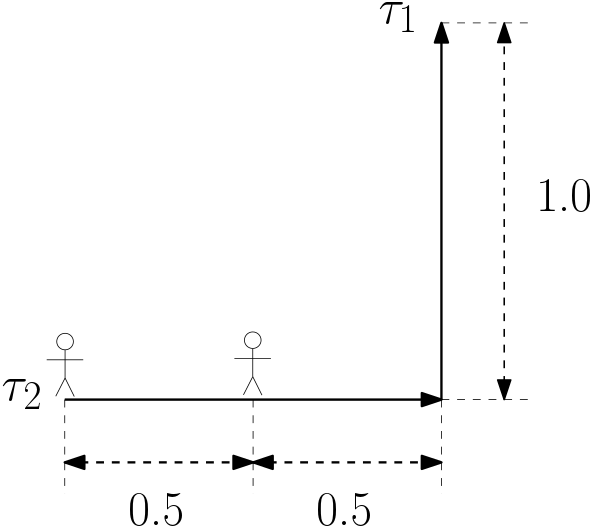
\includegraphics[width=.4\textwidth]{01/04}
\end{figure}

Two agents (agent 1 on the left and agent 2 on the right) are concurring for the acquisition of two tasks: $\tau_1$ and $\tau_2$.\\
It makes no sense for them to acquire just one of the two tasks. Please notice that in order to complete the full task an agent must go to the start of the arrow/task and fully traverse its edge.

Condering all of the above the valuation of the tasks for the two agents can be represented as a cost-to-go:

\begin{gather*}
\text{Agent 1: }\qquad c_1(\tau_1) =2.0 \qquad c_1(\tau_2) =1.0 \qquad c_1(\tau_1, \tau_2) =2.0\\
\text{Agent 2: }\qquad c_2(\tau_1) = 1.5  \qquad c_2(\tau_2) = 1.5 \qquad c_2(\tau_1, \tau_2) =2.5 
\end{gather*}
However if both agents decided to follow this strategy, task $\tau_1$ would go to agent 2 (lower cost to go), whereas task $\tau_2$ would go to agent 1 (lower cost to go).

In order for agent 1 to win both tasks, since it is of no use for an agent to win just one task in an interrelated auction, it can incorporate the full look ahead in its bid.

If in fact, agent 1 wins $\tau_1$, it will bid $c_1(\tau_2) = c_1(\tau_1, \tau_2) - c_1(\tau_1) = 0$ for the second task, otherwise it will bid $c_1(\tau_2) = 1$.
So it makes sense to accomodate the first bid with this knowledge.
If agent 1 wins $\tau_1$, it will win $\tau_2$ at the price of 0 and gets a payoff of $c_1(\tau_2) - 0 = 1$ that can redistribute to the first bid.

In conclusion the dominant strategy is to accomodate the payoff into the first bid:
\[c_1(\tau_1) -payoff = 2-1=1\]

In other terms this implies that if agent 1 realizes that by winning $\tau_2$ it will automatically win $\tau_1$, it will bid ``higher'' for $\tau_1$ or say that the effort to complete task $\tau_1$ will be lower by winning also  $\tau_2$. 

\subsection{Lies and Collusion}
It is in the auctioneer interest to have a protocol that is immune to collusion by bidders, i.e. that made it against the bidder' best interests to engage in collusion with other bidders.

Similarly, as a potential bidder in an auction, we would like a protocol that made honesty on the part of the auctioneer the dominant strategy.

None of the auction discussed above is immune to collusion: for any of them the grand coalition of all agents involved in bidding for the good can agree beforehand to collude to put forward artificially low bids for the good on offer.\\
When the good is obtaines, the bidders can then obtain its true value and split the profits among themselves.
A solution to collusion of the bidder is to modify the protocol so that the bidders cannot identify each other which however it's not possible in open cry auctions.

With regard to the honesty of the auctioneer, the main opportunity for lying occurs in the Vickrey auctions: the auctioneer can lie to the winner about the price of the second highest bid. A solution to this is to sign bids in some way so that the winner can independently verify the value of the second highest bid ro use a trusted third party to handle bids.

In open cry auctino settings there is no possibility for lying by the auctioneer, nor in  the first-price sealed-bid auctions.

Lastly, another possible opportunity for lying by the auctioneer is to place bogus bidders (aka \side{shills}), in an attempt to artificially inflate the current bidding price.

Moreover, there are main limitation of auctions is that they are only concerned with the allocation of goods and as such are not adequate for settling agreements that concerns maters of mutual interest.

\section{Contract Net Protocol (CNP)}

\section{Negotiation parameters}
The basic components that make up a negotiation setting are:
\begin{itemize}
\item A \side{Negotiation set}, which represents the space of possible proposals that agents can make
\item A \side{protocol}, which defines the legal proposals that agents can make, as a funciton of prior negotiation history.
\item A collection of \side{strategies}, one for each agent, which determine what proposals the agents will make.
\item A \side{rule} that determines when a deal has been struck, and what this agreement deal is.
\end{itemize}

Negotiation usually proceeds in a series of rounds, with some proposal made at every round. The proposals that agents make are defined by their strategy, must be drawn from the negotiation set, and must be legal, as defined by the protocol.\\
If agreement is reaches, as defined by the agreement rule, then negotiation terminates with the agreement deal.\\

Several attributes may complicate negotiation:
\begin{itemize}
\item Multiple issues are involved: in case of a single attribute/price we have a symmetric scenario which is easy to analyze because it is always obvious what represents a concession.

On the other hand, in multiple-issue negotiation scenarios, agents negotiate over not just the value of a single attribute, but the values of multiple attributes, which may be interrelated. In such scenarios, it is usually much less obvious what represents a true concession.

Moreover multiple attributes also lead to an exponential growth in the space of possible deals. This means that, in attempting to decide what proposal to make next, it will be entirely unfeasible for an agent to explicitly consider every possible deal in domains of moderate size.
\item Another source of complexity in negotiation is the number of agents involved in the process, and the way in which these agents interact. There are three obvious possibilities:
\begin{enumerate}
\item \side{One-to-one negotiation}
\item \side{Many-to-one negotiation}, as in the case of auctions or reverse auctions
\item \side{Many-to-many negotiation}
\end{enumerate}
\end{itemize}

\subsection{Task Oriented Domain}
The idea behind Negotiation for task allocation is that agents who have tasks to carry out may be able to benefit by reorganizing the distribution of tasks among themselves; but this raises the issue of how to reach agreement on who will do which tasks.

Formally this scenario is known under the name of \side{Task Oriented Domain (TOD)}. A task oriented domain is a triple:
\[< T, Ag, c >\]
where
\begin{itemize}
\item $T$ is the finite set of all possible tasks
\item $Ag = \{1,...,n\}$ is the finite set of negotiation participant agents
\item $c: 2^T \rightarrow\mathbb{R}_+$ is a function which defines the cost of executing each subset of tasks: the cost of executing any set of tasks is a positive real number 
\end{itemize}

The cost functino must satisfy two constraints:
\begin{enumerate}
\item It must be \side{monotonic}
\[\text{If } T_1, T_2 \subseteq T \text{ are sets of tasks such that } T_1\subseteq T_2, then c(T_1) \le c(T_2)\]
\item The cost of doing nothing is zero
\[c(0) =0\]
\end{enumerate}

We will restrict our attention as follows:
\begin{itemize}
\item One-to-one negotiation scenario, with two agents $\{1,2\}$
\item Given an encounter $< T_1, T_2>$, a \side{deal} will be an allocation of the tasks $T_1 \cup T_2$ to the agents 1 and 2.
\item Three types of deal may happen under this conditions:
\begin{enumerate}
\item \side{Pure deals}: agents are deterministically allocated exhaustive disjoint task set.\\
Formally, a pure deal is a pair $< D_1, D_2>$ where 
\[D_1 \cup D_2 = T_1 \cup T_2\]
\item \side{Mixed deals}: specify a probability distribution over partitions
\item \side{All-or-Nothing deals}: mixed deals where the alternatives only include partitions where one agent handles the tasks of all agents.
\end{enumerate}
\item The \side{cost} to an agent $i$ of a deal $\delta = <D_1, D_2>$ is defined to be $c(D_i)$ and it will  be denoted as $cost_i(\delta)$
\item The \side{utility} of a deal $\delta$ to an agent $i$ is the difference between the cost of agent $i$ doing the tasks $T_i$ that it was originally assigned in the encounter and the cost $cost_i(\delta)$ of the tasks it is assigned in $\delta$:
\[utility_i(\delta) = c(T _i) - cost_i(\delta)\]
Thus the utility of a deal represents how much the agent has to gain from the deal (a negative utility means that the agent is worse off than it was originally)
\item If the agents fail to reach an agreement they must perform the tasks that they were originally allocated (\side{conflict deal}, $\Theta = <T_1, T_2>$) 
\end{itemize} 
The properties that govern this agent interactions are:
\begin{itemize}
\item Dominance\\
A deal $\delta_1$ is said to be dominant if and only if:
\begin{enumerate}
\item Deal $\delta_1$ is at least as good for every agent as $\delta_2$
\[\forall i \in \{1,2\}, utility_i(\delta_1) \ge utility_i(\delta_2)\]
\item Deal $\delta_1$ is better for some agent than $\delta_2$
\[\exists i \in \{ utility_i(\delta_1) > utility_i(\delta_2)\}\]
\end{enumerate}
A deal is said to be \side{weakly dominant} if at least the first condition holds.
\item Pareto optimal\\
A deal $\delta$ is Pareto optimal if there is no deal $\delta'$ such that $\delta' \cmore \delta$
\item Individual rationality\\
A deal $\delta$ is said to be individual rational if it weakly dominates the conflict deal
\[\delta \cge \Theta\]
If a deal is not individual rational, then at least one agent can do better by simply performing the tasks it was originally allocated (it prefers the conflict deal)
\end{itemize}

Given all of the above, we are in the position to define the space of possible proposals that agents can make: the negotiation set consists of the set of deals that are individual rational and Pareto optimal.\\
In the following figure is proposed the set of possible deals in a 2 agent encounter

\begin{figure}[!h]
\centering 
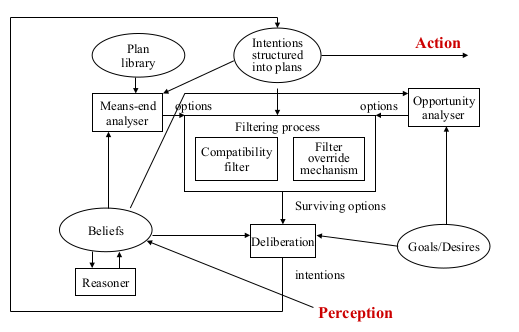
\includegraphics[width=.5\textwidth]{01/05}
\end{figure}
Here, the first, third and fourth quadrant includes the subset of deals that are not individual rational. (there is no point for an agent to accept a deal that produces negative utility).\\
Similarly, all deals strictly inside the ellipsis are not Pareto Optimal. Which brings as to the boundary of the negotiation set in the second quadrant.\\
Agent $i$ (ordinate axis) will start at its best possible deal (B), whereas agent $j$ (abscissa axis) will start at its best possible deal (C).\\
Both agent will then concede in one or more rounds until a point of mutual agreement on the boundary of the negotiation set is reached.

\subsection{Worth Oriented Domain}
\subsection{Monotonic Concession Protocol (MCP)}
The rules of this negotiation protocol are:
\begin{itemize}
\item Negotiation proceeds in a series of rounds
\item On the first round both agents simultaneously propose a deal from the negotiation set
\item An agreement is reached if the two agents propose deals $\delta_1$ and $\delta_2$, respectively, such that either:
\[utility_1(\delta_2) \ge utility_1(\delta_1)\qquad || \qquad utility_2(\delta_1)\ge utility_2(\delta_2)\]
\item If both agents offers match or exceed those of the other agent, then one of the proposals is selected at random
\item If only one proposal exceeds or matches the other's proposal, then this is the agreement deal
\item If no agreement is reached, then negotiation proceeds to another round of simultaneous proposals, where no agent is allowed to make a proposal that is less preferred by the other agent than the deal it proposed at the previous round
\item If neither agent makes a concession in some round, then negotiation terminates with the conflict deal
\end{itemize}

Using such protocol negotiation is guaranteed to end (with or without agreement) after a finite number of rounds, however the protocol does not guarantee that the agreement (or lack of it) will be reached quickly.
\subsection{The Zeuthen strategy}
\begin{enumerate}
\item What should an agent's first proposal be?
\item On any given round, who should concede?
\item If an agent concedes, then how much should it concede?
\end{enumerate}

With regard to the first question: an agent's first proposal should be its most preferred deal.

With respect to the second question: the idea of the \side{Zeuthen strategy} is to measure an agent's willingness to risk conflict (i.e. an agent is more willing to risk conflict if the difference in utility between its current proposal and the conflict deal is low).

Agent $i$'s willingness to risk conflict at round $t$ is:
\[risk^t_i = \cfrac{\text{utilty }i\text{ loses by conceding and accepting}j\text{`s offer} }{\text{utility }i\text{loses by not conceding and causing conflict}}\]
Until an agreement is reached, the value of risk is between 0 and 1 (the higher the value the higher the risk, which means that an agent has less to lose from conflict and as such it is more willing to risk conflict).\\
Formally:
\[risk^t_i =
\begin{dcases}
1 & \text{If }utility_i(\delta_i^t)=0\\
\cfrac{utility_i(\delta_i^t) - utility_i(\delta_j^t)}{utility_i(\delta_i^t)} &\text{otherwise}
\end{dcases}
\]
Hence, the zeuthen strategy proposes that the agent to concede on round $t$ of negotiation should be the one with the smaller value of risk.\\
Moreover, the agent in question should make the smallest concession necessary to change the balance of risk, so that on the next round, the other agent will concede.

Lastly, in the case of equal risk, a coin flip will decide which agent should concede, otherwise we are in the same situation of the prisoner's dilemma.

We notice that the Zeuthen strategy and the protocol itself:
\begin{itemize}
\item Does not guarantee success, but it does guarantee termination
\item It does not guarantee to maximize social welfare
\item If agreement is reached, then this agreement will be Pareto Optimal
\item It is individual rational
\item It is in Nash equilibrium (if an agent is using the Zeuthen strategy the other can do no better than using the same strategy)
\end{itemize}
\subsection{Deception}